A DenseNet121 modell sb-photothemes-imagenet114 adathalmazon teljes tanítással történt tesztelésének eredménye. Lásd a soron következő ábrákat és táblázatokat a mérések eredményeihez.

\subsubsection{DenseNet121 teljes tanítás folyamata}
\begin{itemize} 
  \item Epoch 1/10 - train: 2259/2259 [04:29<00:00,  8.38it/s]
  \item Epoch 1/10 - val: 282/282 [00:24<00:00, 11.34it/s]
  \item Epoch 1: Train loss=1.6432, acc=0.5788, Val loss=1.2331, acc=0.6573
  \item Epoch 2/10 - train: 2259/2259 [04:29<00:00,  8.39it/s]
  \item Epoch 2/10 - val: 282/282 [00:24<00:00, 11.36it/s]
  \item Epoch 2: Train loss=1.0401, acc=0.7057, Val loss=1.0652, acc=0.7020
  \item Epoch 3/10 - train: 2259/2259 [04:30<00:00,  8.36it/s]
  \item Epoch 3/10 - val: 282/282 [00:24<00:00, 11.38it/s]
  \item Epoch 3: Train loss=0.7765, acc=0.7751, Val loss=0.9971, acc=0.7206
  \item Epoch 4/10 - train: 2259/2259 [04:30<00:00,  8.36it/s]
  \item Epoch 4/10 - val: 282/282 [00:26<00:00, 10.57it/s]
  \item Epoch 4: Train loss=0.5863, acc=0.8264, Val loss=1.0337, acc=0.7208
  \item Epoch 5/10 - train: 2259/2259 [04:30<00:00,  8.35it/s]
  \item Epoch 5/10 - val: 282/282 [00:24<00:00, 11.36it/s]
  \item Epoch 5: Train loss=0.4442, acc=0.8663, Val loss=1.0095, acc=0.7380
  \item Epoch 6/10 - train: 2259/2259 [04:29<00:00,  8.37it/s]
  \item Epoch 6/10 - val: 282/282 [00:24<00:00, 11.30it/s]
  \item Epoch 6: Train loss=0.3490, acc=0.8949, Val loss=1.0286, acc=0.7421
  \item Epoch 7/10 - train: 2259/2259 [04:29<00:00,  8.39it/s]
  \item Epoch 7/10 - val: 282/282 [00:24<00:00, 11.38it/s]
  \item Epoch 7: Train loss=0.2790, acc=0.9152, Val loss=1.0950, acc=0.7380
  \item Epoch 8/10 - train: 2259/2259 [04:29<00:00,  8.37it/s]
  \item Epoch 8/10 - val: 282/282 [00:25<00:00, 11.25it/s]
  \item Epoch 8: Train loss=0.2366, acc=0.9282, Val loss=1.1248, acc=0.7423
  \item Epoch 9/10 - train: 2259/2259 [04:30<00:00,  8.34it/s]
  \item Epoch 9/10 - val: 282/282 [00:25<00:00, 11.17it/s]
  \item Epoch 9: Train loss=0.2048, acc=0.9372, Val loss=1.1491, acc=0.7373
  \item Epoch 10/10 - train: 2259/2259 [04:29<00:00,  8.37it/s]
  \item Epoch 10/10 - val: 282/282 [00:25<00:00, 11.20it/s]
  \item Epoch 10: Train loss=0.1791, acc=0.9451, Val loss=1.1960, acc=0.7377
  \end{itemize}

\subsubsection{DenseNet121 teljes tanítás folyamata}
  \begin{figure}[H]
    \centering
    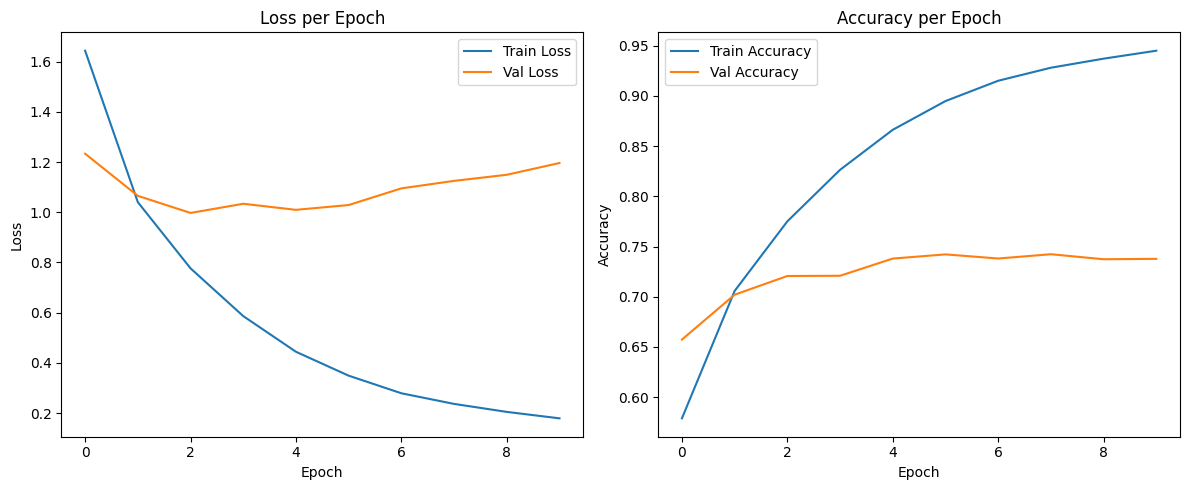
\includegraphics[width=1.0\textwidth]{images/phase02/DenseNet121_learning_curve.png}
    \caption{DenseNet121 teljes tanítás utáni sima Confusion Mátrix}
    \label{fig:phase02_DenseNet121_learning_curves}
  \end{figure}

\subsubsection{DenseNet121 teljes tanítás utáni eredményei}
  \begin{center}
  \begin{longtable}{l c}
  \caption{DenseNet121 teljes tanítás utáni vizsgálati eredményei} \label{tab:phase02_DenseNet121} \\
  \toprule
  \textbf{Metrika} & \textbf{Érték} \\
  \midrule
  \endfirsthead
  \toprule
  \textbf{Metrika} & \textbf{Érték} \\
  \midrule
  \endhead
  Top-1 Accuracy & 0.7400 \\
  Top-5 Accuracy & 0.9266 \\
  Precision & 0.6811 \\
  Recall & 0.6808 \\
  F1-score & 0.6696 \\
  Inference time & 25.23 sec \\
  \bottomrule
  \end{longtable}
  \end{center}

\subsubsection{DenseNet121 eredményeinek összehasonlítása}
  \begin{center}
  \begin{longtable}{l c c}
  \caption{DenseNet121 eredményeinek összehasonlítása} \label{tab:phase02_DenseNet121_compare} \\
  \toprule
  \textbf{Metrika} & \textbf{Pretrained} & \textbf{Fine-tuned} \\
  \midrule
  \endfirsthead
  \toprule
  \textbf{Metrika} & \textbf{Pretrained} & \textbf{Fine-tuned} \\
  \midrule
  \endhead
  Top-1 Accuracy  & 0.4498 & 0.7400 \\
  Top-5 Accuracy & 0.7806 & 0.9266 \\
  Precision & 0.3874 & 0.6811 \\
  Recall & 0.3611 & 0.6680 \\
  F1-score & 0.3408 & 0.6696 \\
  Inference time & 25.15 sec & 25.23 sec \\
  \bottomrule
  \end{longtable}
  \end{center}

\subsubsection{DenseNet121 eredményeinek összehasonlítása}
  \begin{figure}[H]
    \centering
    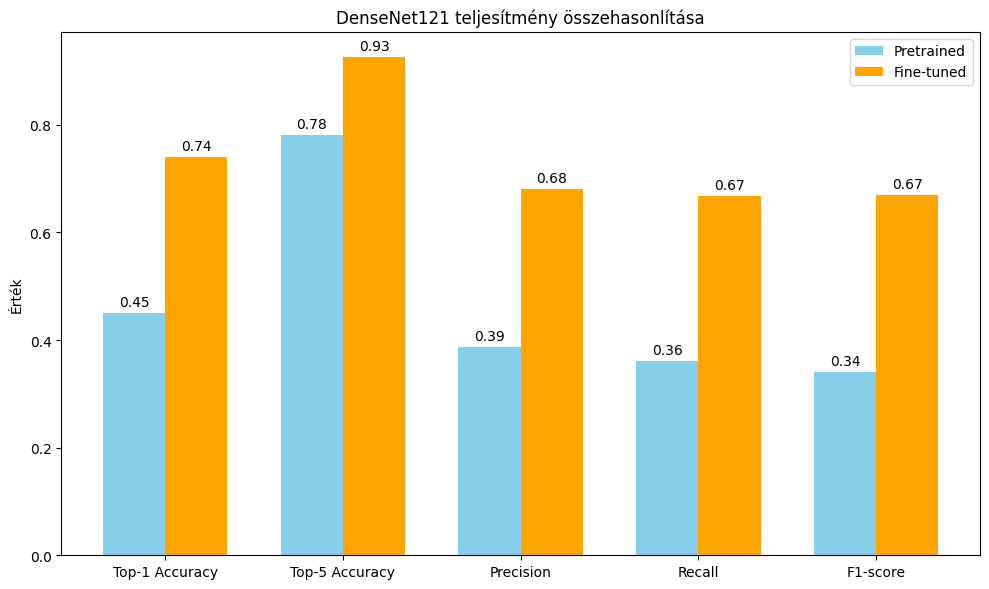
\includegraphics[width=1.0\textwidth]{images/phase02/DenseNet121_compare01.png}
    \caption{DenseNet121 eredményeinek összehasonlítása}
    \label{fig:DenseNet121_compare01}
  \end{figure}

\subsubsection{DenseNet121 eredményeinek összehasonlítása}
  \begin{figure}[H]
    \centering
    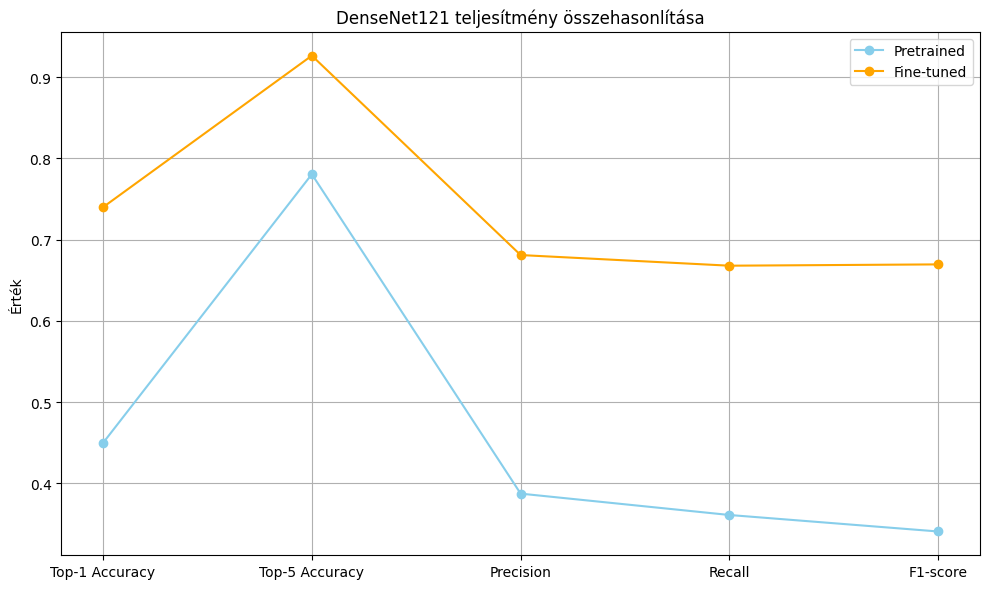
\includegraphics[width=1.0\textwidth]{images/phase02/DenseNet121_compare02.png}
    \caption{DenseNet121 eredményeinek összehasonlítása}
    \label{fig:DenseNet121_compare02}
  \end{figure}

\subsubsection{DenseNet121 teljes tanítás utáni sima Confusion Mátrix}
  \begin{figure}[H]
    \centering
    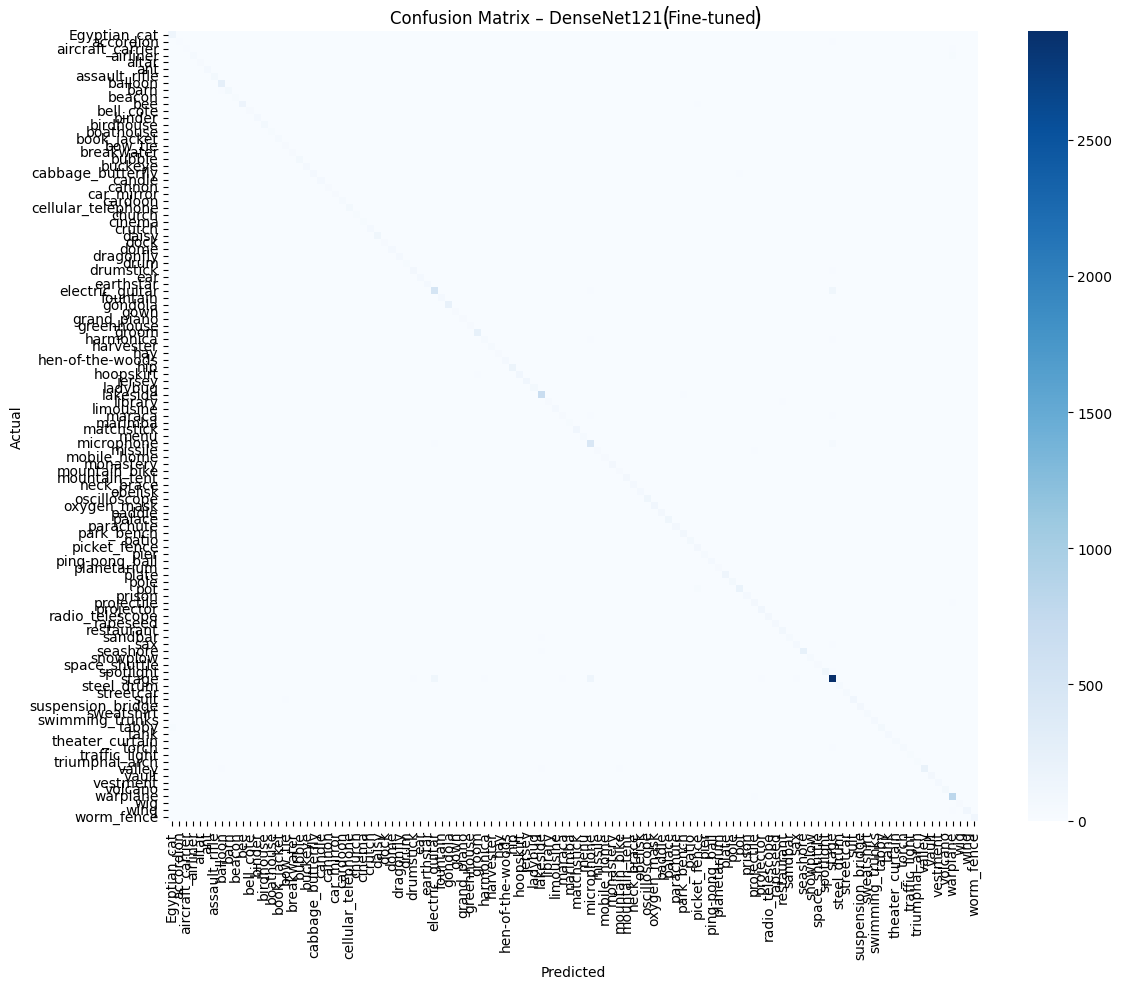
\includegraphics[width=1.0\textwidth]{images/phase02/phase02_DenseNet121_basic_conf_mat.png}
    \caption{DenseNet121 teljes tanítás utáni sima Confusion Mátrix}
    \label{fig:phase02_DenseNet121_basic_conf_mat}
  \end{figure}

  \subsubsection{DenseNet121 Confusion Mátrixok összehasonlítása}
  \begin{figure}[H]
    \centering
    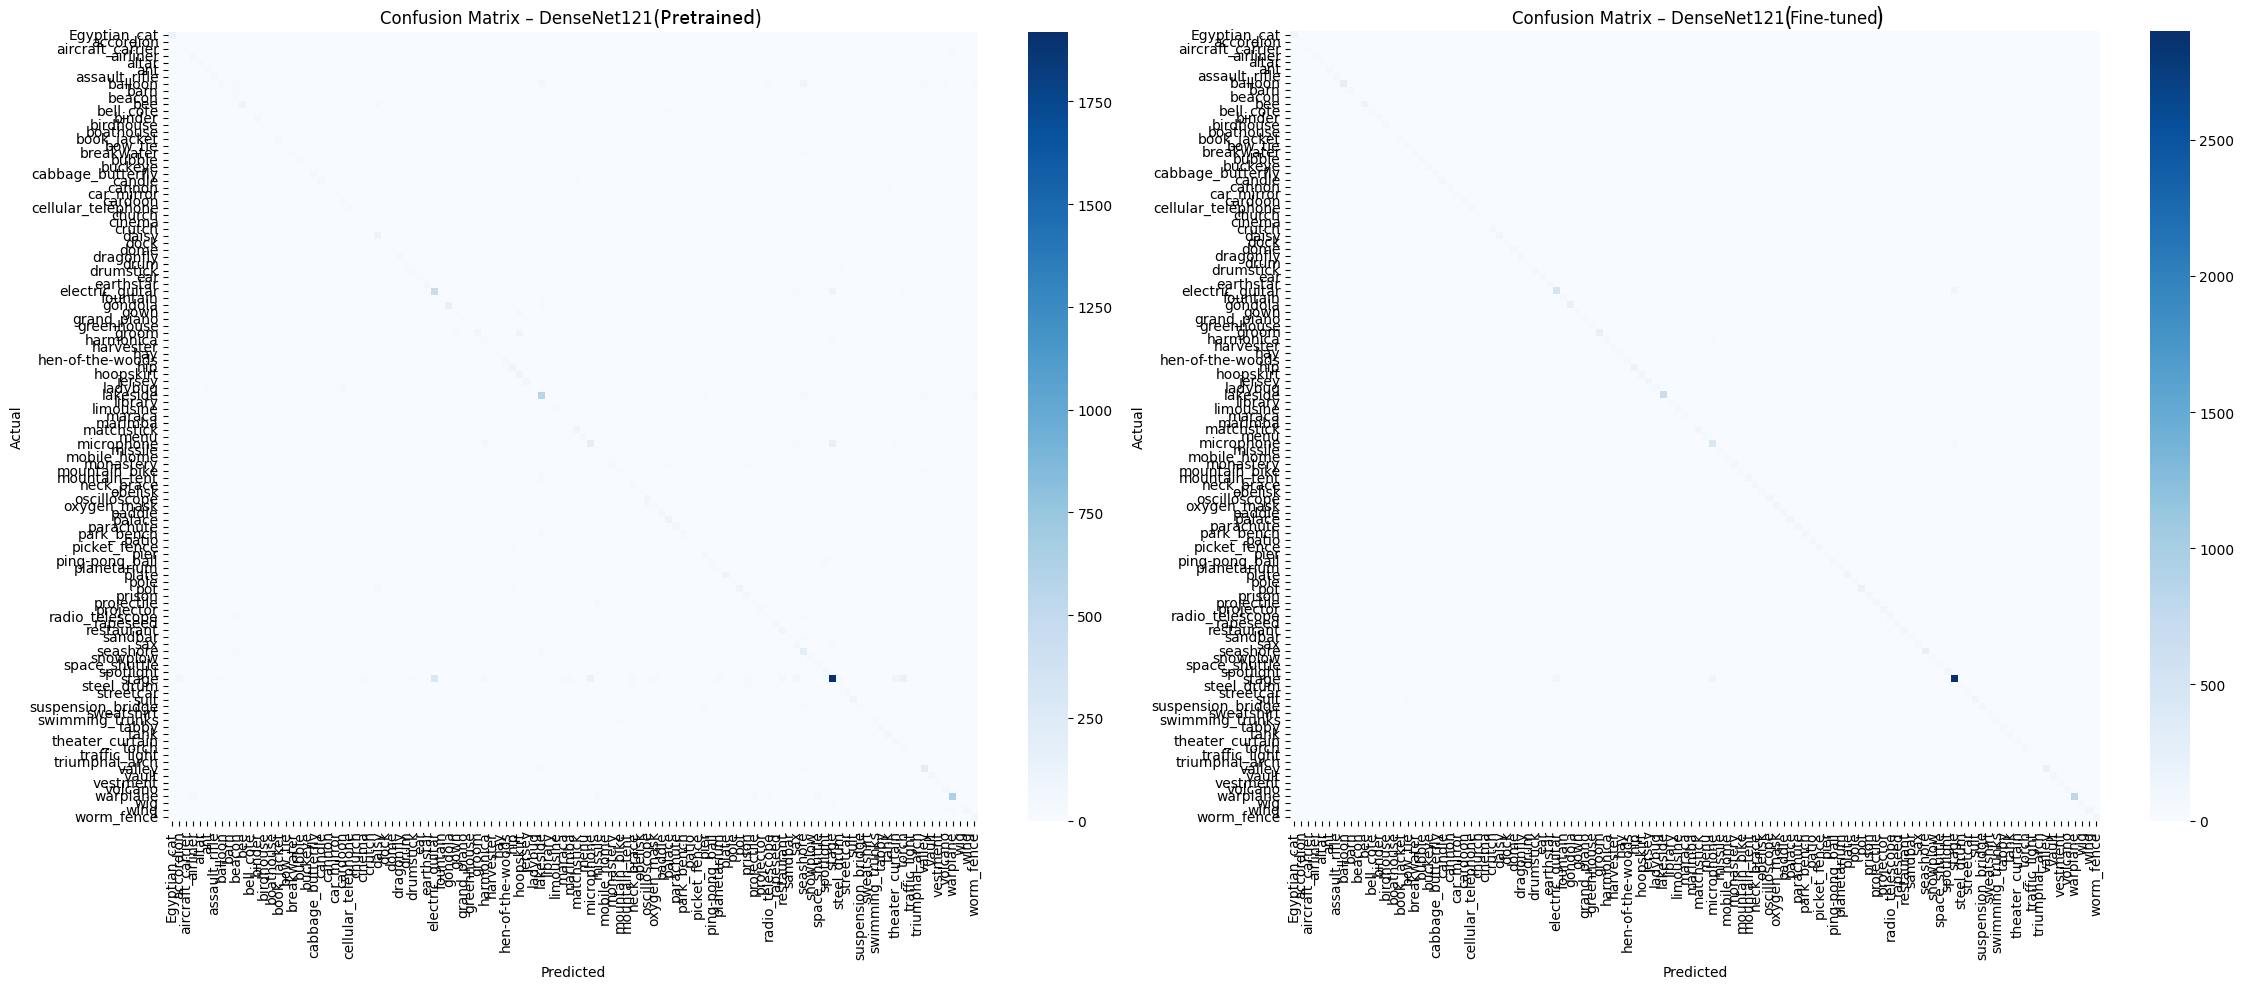
\includegraphics[width=1.0\textwidth]{images/phase02/phase02_DenseNet121_basic_conf_mat_compare.png}
    \caption{DenseNet121 sima Confusion Mátrixok összehasonlítása}
    \label{fig:phase02_DenseNet121_basic_conf_mat_compare}
  \end{figure}

  \subsubsection{DenseNet121 teljes tanítás utáni normalizált Confusion Mátrix}
  \begin{figure}[H]
    \centering
    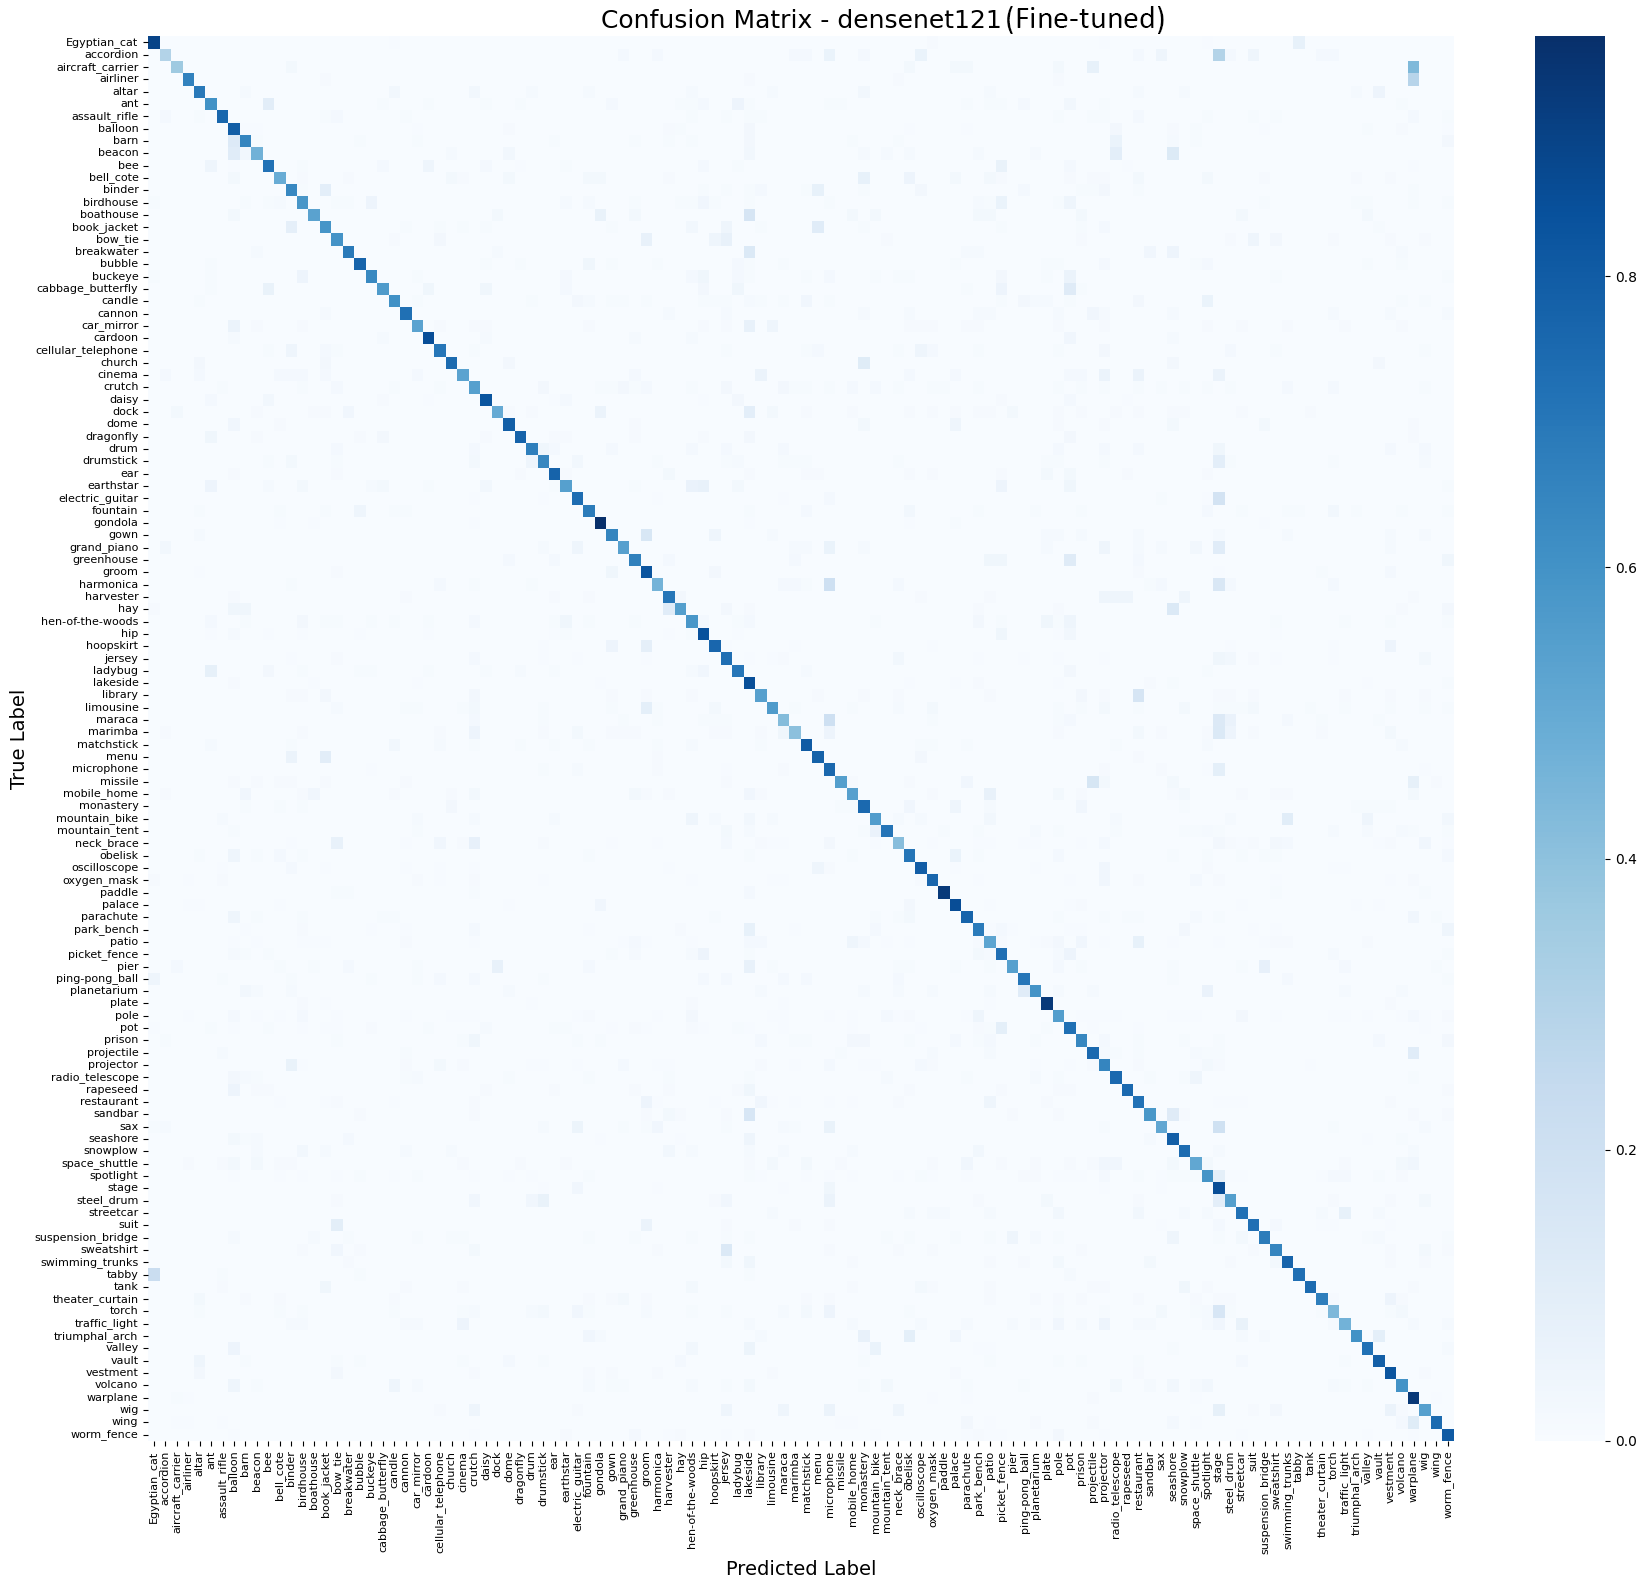
\includegraphics[width=1.0\textwidth]{images/phase02/phase02_DenseNet121_normalised_conf_mat.png}
    \caption{DenseNet121 teljes tanítás utáni normalizált Confusion Mátrix}
    \label{fig:phase02_DenseNet121_normalised_conf_mat}
  \end{figure}

  \subsubsection{DenseNet121 normalizált Confusion Mátrixok összehasonlítása}
  \begin{figure}[H]
    \centering
    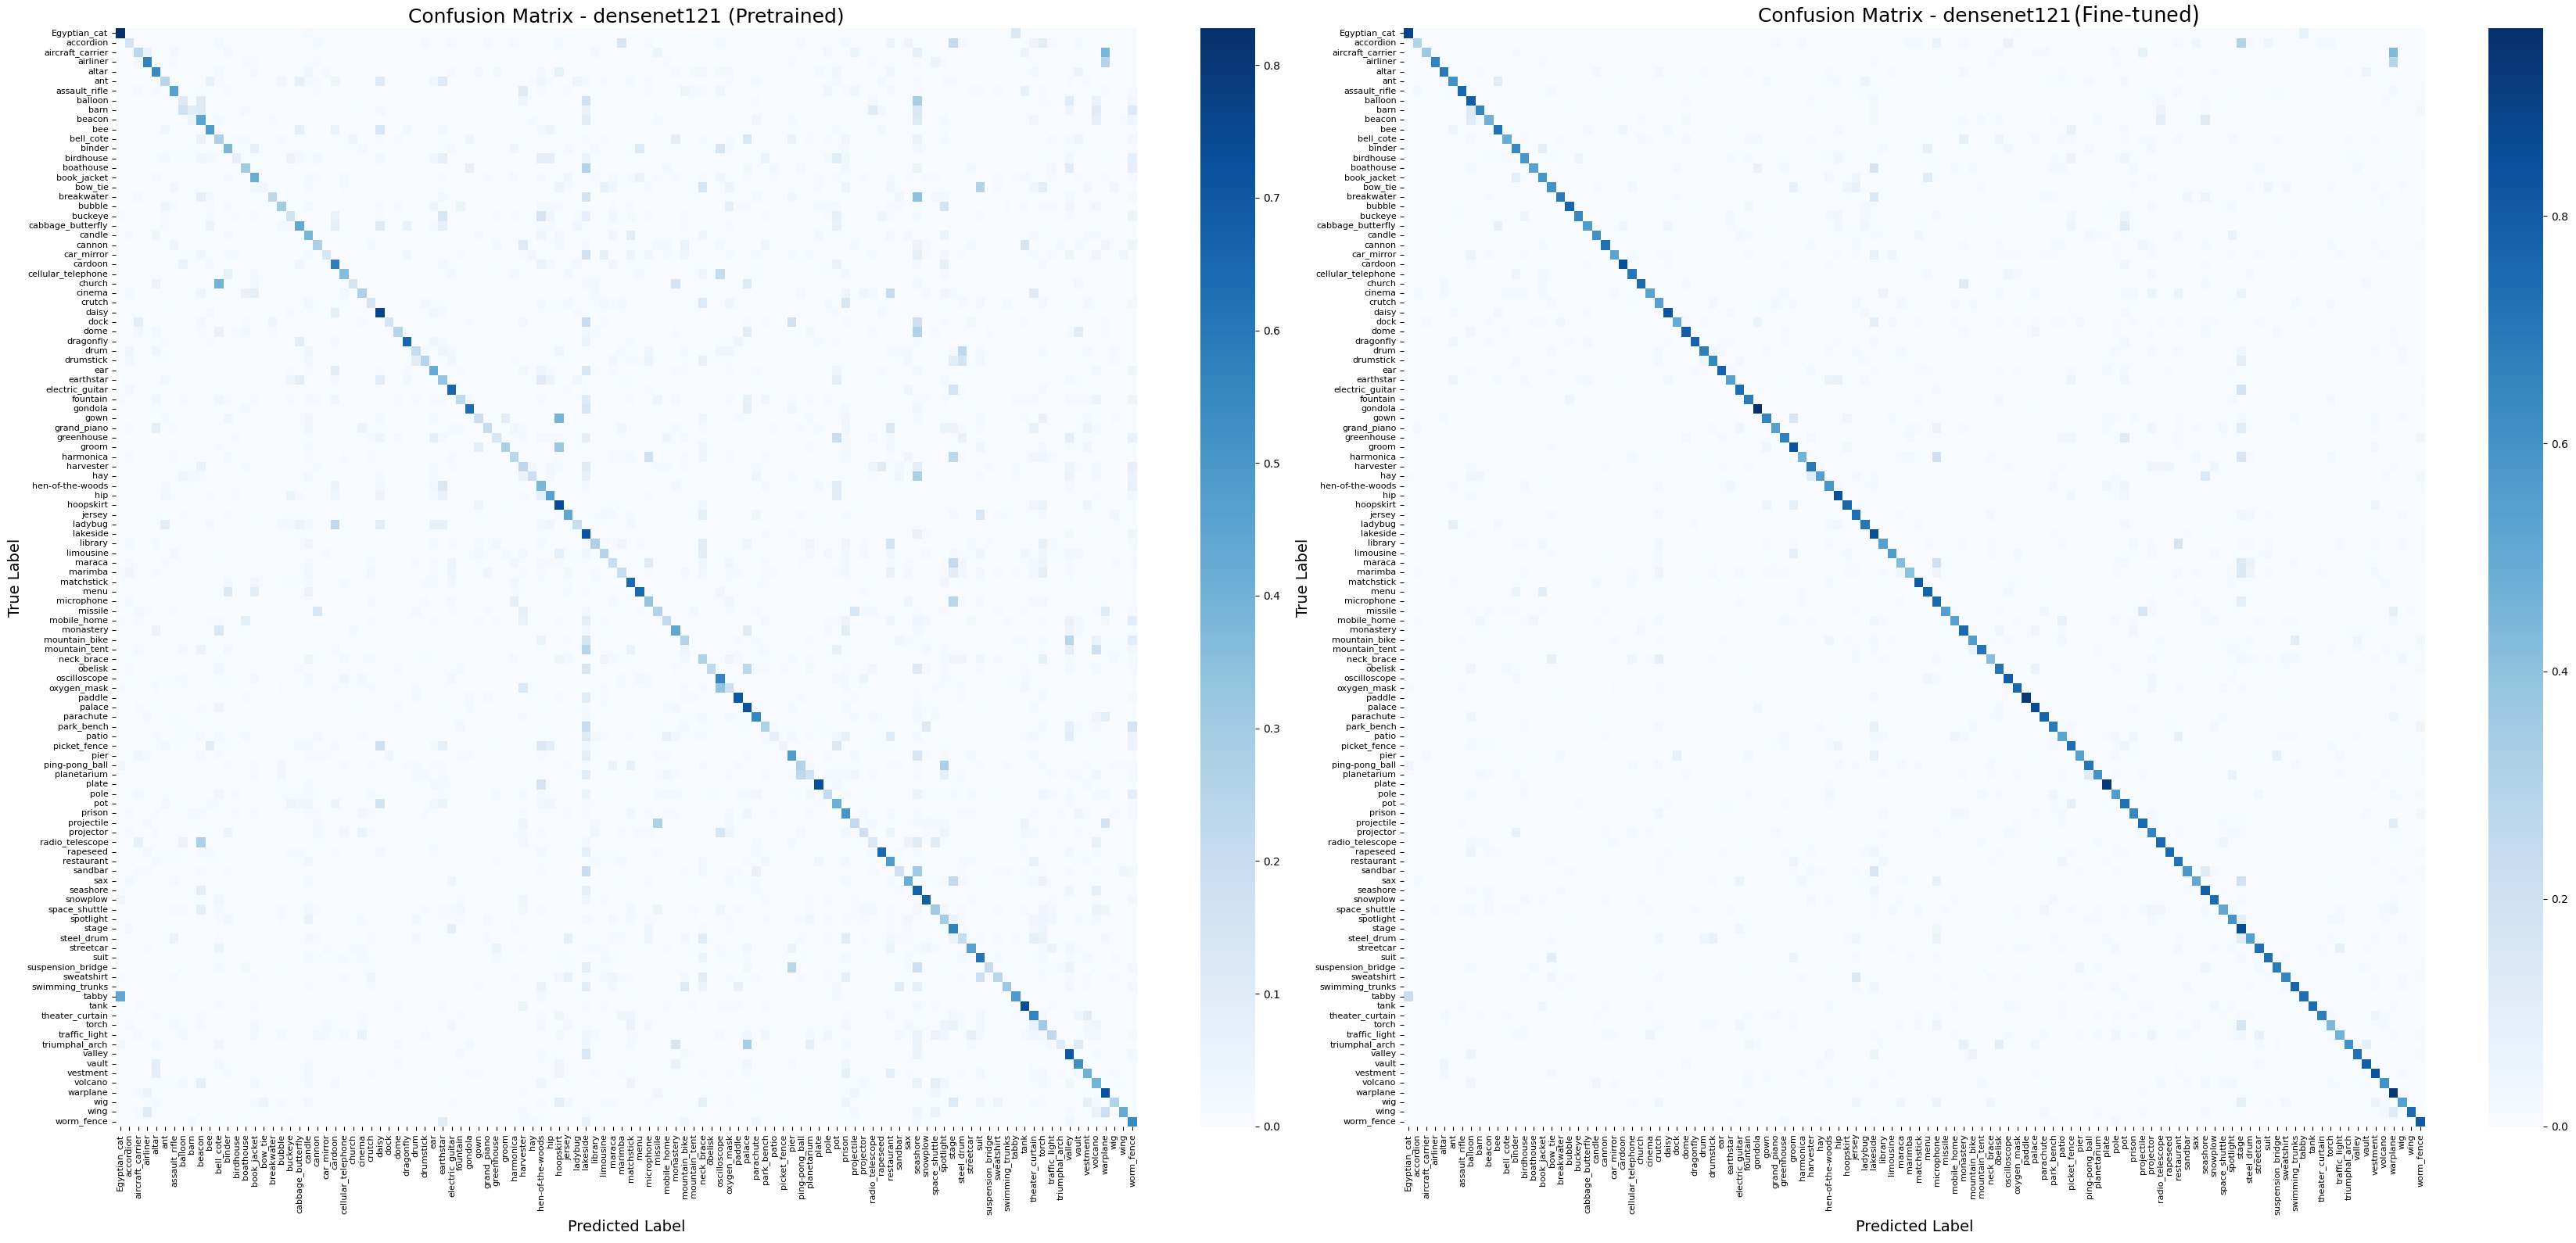
\includegraphics[width=1.0\textwidth]{images/phase02/phase02_DenseNet121_normalised_conf_mat_compare.png}
    \caption{DenseNet121 normalizált Confusion Mátrixok összehasonlítása}
    \label{fig:phase02_DenseNet121_normalised_conf_mat_compare}
  \end{figure}

\subsubsection{DenseNet121 teljes tanítás utáni részletes osztályonkénti metrikák}
  \begin{center}
\begin{longtable}{lllll}
\caption{DenseNet121 teljes tanítás utáni részletes osztályonkénti metrikák}\label{tab:phase2_DenseNet121_class_table}\\
\toprule
class & precision & recall & f1-score & support \\
\midrule
\endfirsthead
\toprule
class & precision & recall & f1-score & support \\
\midrule
\endhead
tank & 0.94 & 0.74 & 0.83 & 78 \\
wing & 0.93 & 0.74 & 0.83 & 148 \\
paddle & 0.92 & 0.92 & 0.92 & 93 \\
gondola & 0.90 & 0.96 & 0.93 & 227 \\
stage & 0.89 & 0.86 & 0.87 & 3380 \\
valley & 0.89 & 0.72 & 0.80 & 295 \\
dragonfly & 0.88 & 0.77 & 0.82 & 75 \\
rapeseed & 0.88 & 0.75 & 0.81 & 77 \\
warplane & 0.88 & 0.93 & 0.91 & 871 \\
mountain-tent & 0.87 & 0.71 & 0.78 & 121 \\
tabby & 0.87 & 0.73 & 0.79 & 107 \\
missile & 0.86 & 0.54 & 0.66 & 82 \\
plate & 0.86 & 0.93 & 0.90 & 143 \\
airliner & 0.85 & 0.66 & 0.75 & 80 \\
bubble & 0.85 & 0.77 & 0.81 & 100 \\
daisy & 0.84 & 0.83 & 0.83 & 149 \\
assault-rifle & 0.83 & 0.76 & 0.79 & 91 \\
lakeside & 0.82 & 0.85 & 0.83 & 801 \\
triumphal-arch & 0.82 & 0.60 & 0.69 & 55 \\
suit & 0.81 & 0.73 & 0.77 & 141 \\
bee & 0.80 & 0.72 & 0.76 & 212 \\
cabbage-butterfly & 0.80 & 0.56 & 0.66 & 101 \\
oscilloscope & 0.80 & 0.80 & 0.80 & 143 \\
suspension-bridge & 0.80 & 0.69 & 0.74 & 127 \\
Egyptian-cat & 0.79 & 0.89 & 0.84 & 145 \\
ear & 0.79 & 0.78 & 0.78 & 80 \\
hoopskirt & 0.79 & 0.76 & 0.78 & 135 \\
pier & 0.79 & 0.55 & 0.65 & 97 \\
dome & 0.78 & 0.79 & 0.78 & 85 \\
hip & 0.78 & 0.84 & 0.81 & 195 \\
oxygen-mask & 0.78 & 0.76 & 0.77 & 143 \\
vault & 0.78 & 0.79 & 0.78 & 104 \\
electric-guitar & 0.77 & 0.74 & 0.75 & 687 \\
groom & 0.77 & 0.83 & 0.80 & 285 \\
matchstick & 0.77 & 0.80 & 0.79 & 127 \\
buckeye & 0.76 & 0.63 & 0.69 & 101 \\
dock & 0.76 & 0.50 & 0.60 & 84 \\
cellular-telephone & 0.75 & 0.70 & 0.73 & 104 \\
candle & 0.74 & 0.60 & 0.66 & 111 \\
limousine & 0.74 & 0.56 & 0.64 & 119 \\
palace & 0.74 & 0.86 & 0.80 & 139 \\
ping-pong-ball & 0.74 & 0.70 & 0.72 & 91 \\
seashore & 0.74 & 0.79 & 0.76 & 289 \\
earthstar & 0.73 & 0.55 & 0.63 & 121 \\
parachute & 0.73 & 0.77 & 0.75 & 117 \\
barn & 0.72 & 0.65 & 0.68 & 111 \\
church & 0.72 & 0.74 & 0.73 & 35 \\
ladybug & 0.72 & 0.70 & 0.71 & 108 \\
swimming-trunks & 0.72 & 0.77 & 0.74 & 79 \\
theater-curtain & 0.72 & 0.69 & 0.71 & 80 \\
balloon & 0.71 & 0.79 & 0.75 & 338 \\
hay & 0.71 & 0.55 & 0.62 & 73 \\
breakwater & 0.70 & 0.69 & 0.70 & 58 \\
cardoon & 0.69 & 0.85 & 0.76 & 55 \\
altar & 0.68 & 0.69 & 0.69 & 59 \\
monastery & 0.68 & 0.75 & 0.71 & 112 \\
pot & 0.68 & 0.72 & 0.70 & 254 \\
projectile & 0.67 & 0.75 & 0.71 & 117 \\
radio-telescope & 0.67 & 0.74 & 0.70 & 108 \\
sandbar & 0.67 & 0.58 & 0.62 & 83 \\
worm-fence & 0.67 & 0.80 & 0.73 & 137 \\
cannon & 0.66 & 0.73 & 0.69 & 55 \\
volcano & 0.66 & 0.60 & 0.63 & 119 \\
microphone & 0.65 & 0.76 & 0.70 & 596 \\
spotlight & 0.65 & 0.59 & 0.62 & 202 \\
bell-cote & 0.64 & 0.49 & 0.56 & 77 \\
boathouse & 0.64 & 0.53 & 0.58 & 43 \\
fountain & 0.64 & 0.68 & 0.66 & 92 \\
menu & 0.64 & 0.78 & 0.70 & 68 \\
park-bench & 0.64 & 0.69 & 0.66 & 144 \\
prison & 0.64 & 0.64 & 0.64 & 101 \\
streetcar & 0.64 & 0.72 & 0.68 & 65 \\
sweatshirt & 0.63 & 0.65 & 0.64 & 80 \\
neck-brace & 0.62 & 0.42 & 0.50 & 137 \\
planetarium & 0.62 & 0.60 & 0.61 & 62 \\
birdhouse & 0.61 & 0.59 & 0.60 & 116 \\
harvester & 0.61 & 0.70 & 0.65 & 71 \\
snowplow & 0.61 & 0.74 & 0.67 & 62 \\
grand-piano & 0.60 & 0.54 & 0.57 & 63 \\
jersey & 0.60 & 0.73 & 0.66 & 154 \\
binder & 0.59 & 0.64 & 0.61 & 105 \\
patio & 0.59 & 0.52 & 0.55 & 144 \\
torch & 0.59 & 0.44 & 0.50 & 116 \\
car-mirror & 0.58 & 0.53 & 0.55 & 68 \\
drumstick & 0.58 & 0.64 & 0.61 & 126 \\
mobile-home & 0.58 & 0.54 & 0.56 & 83 \\
ant & 0.57 & 0.60 & 0.58 & 95 \\
greenhouse & 0.57 & 0.67 & 0.61 & 51 \\
marimba & 0.57 & 0.41 & 0.47 & 79 \\
obelisk & 0.57 & 0.71 & 0.63 & 95 \\
restaurant & 0.57 & 0.72 & 0.63 & 141 \\
book-jacket & 0.56 & 0.59 & 0.58 & 90 \\
library & 0.56 & 0.54 & 0.55 & 74 \\
vestment & 0.56 & 0.83 & 0.67 & 69 \\
sax & 0.55 & 0.51 & 0.53 & 112 \\
gown & 0.54 & 0.65 & 0.59 & 66 \\
space-shuttle & 0.54 & 0.51 & 0.53 & 84 \\
traffic-light & 0.54 & 0.47 & 0.50 & 58 \\
cinema & 0.53 & 0.53 & 0.53 & 51 \\
drum & 0.53 & 0.67 & 0.59 & 49 \\
aircraft-carrier & 0.52 & 0.36 & 0.42 & 39 \\
pole & 0.52 & 0.55 & 0.54 & 136 \\
beacon & 0.51 & 0.47 & 0.49 & 62 \\
projector & 0.51 & 0.65 & 0.57 & 157 \\
steel-drum & 0.51 & 0.55 & 0.53 & 84 \\
hen-of-the-woods & 0.49 & 0.58 & 0.53 & 105 \\
mountain-bike & 0.49 & 0.56 & 0.52 & 66 \\
picket-fence & 0.49 & 0.73 & 0.59 & 118 \\
harmonica & 0.48 & 0.46 & 0.47 & 100 \\
wig & 0.46 & 0.54 & 0.50 & 70 \\
accordion & 0.41 & 0.30 & 0.35 & 47 \\
bow-tie & 0.41 & 0.60 & 0.49 & 67 \\
crutch & 0.40 & 0.54 & 0.46 & 105 \\
maraca & 0.38 & 0.42 & 0.40 & 90 \\
\midrule
accuracy &  &  & 0.74 & 18172 \\
macroavg & 0.68 & 0.67 & 0.67 & 18172 \\
weightedavg & 0.75 & 0.74 & 0.74 & 18172 \\
\bottomrule
\end{longtable}
\end{center}


\subsubsection{GPU memóriahasználat}
\begin{itemize}
  \item aktív GPU: NVIDIA A100-SXM4-40GB
  \item GPU memória (lefoglalt): 1.5 GB
  \item GPU memória (használt):  0.09 GB
\end{itemize}

\subsubsection{Legrosszabbul teljesítő osztályok}
\begin{center}
  \begin{longtable}{llll}
  \caption{Legrosszabbul teljesítő osztályok}\label{tab:phase02_DenseNet121_legrosszabb_osztlyok}\\
  \toprule
  Class & Precision & Recall & F1-score \\
  \midrule
  \endfirsthead
  \toprule
  Class & Precision & Recall & F1-score \\
  \midrule
  \endhead
  maraca & 0.38 & 0.42 & 0.40 \\
  crutch & 0.40 & 0.54 & 0.46 \\
  accordion & 0.41 & 0.30 & 0.35 \\
  bow-tie & 0.41 & 0.60 & 0.49 \\
  wig & 0.46 & 0.54 & 0.50 \\
  harmonica & 0.48 & 0.46 & 0.47 \\
  beacon & 0.51 & 0.47 & 0.49 \\
  aircraft-carrier & 0.52 & 0.36 & 0.42 \\
  marimba & 0.57 & 0.41 & 0.47 \\
  neck-brace & 0.62 & 0.42 & 0.50 \\
  \bottomrule
  \end{longtable}
  \end{center}